\documentclass[12pt]{article}
\usepackage{fancyhdr}
\usepackage{amsmath, enumitem, tikz, pgf}
\usepackage{amssymb, amsmath, graphicx, amsthm, setspace}
\usetikzlibrary{arrows, automata, positioning}
\usepackage[latin1]{inputenc}
\pagestyle{fancy}

\lhead[lh-even]{\textbf{Michael Vu}}  
\lfoot[lf-even]{} 
\chead[ch-even]{\textbf{CSCI 3500 HW 4}}  
\cfoot[cf-even]{} 
\rhead[rh-even]{March 21, 2018}  
\rfoot[rf-even]{}

\begin{document}
	\begin{enumerate}
		\item %1.
		\begin{enumerate}
			\item %a.
				\begin{flalign*}
					S &\Rightarrow X \\
					&\Rightarrow bX \\
					&\Rightarrow bbX \\
					&\Rightarrow bbbX \\
					&\Rightarrow bbb &&
				\end{flalign*}
				
			\item %b.
				\begin{flalign*}
					S &\Rightarrow aS \\
					&\Rightarrow aaS \\
					&\Rightarrow aaX \\
					&\Rightarrow aabX \\
					&\Rightarrow aabbX \\
					&\Rightarrow aabb &&
				\end{flalign*}
				
			\item %c.
				\begin{flalign*}
					S &\Rightarrow X \\
					&\Rightarrow \epsilon &&
				\end{flalign*}
		\end{enumerate}
		
		\item %2.
			\quad \\
			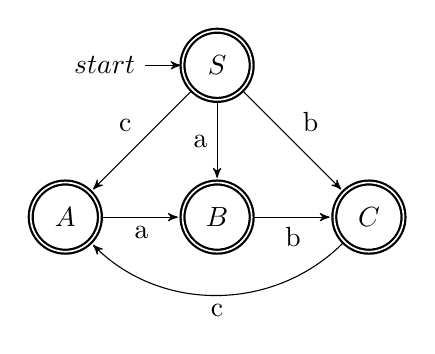
\begin{tikzpicture}
				\tikzset {->, >=stealth', node distance=1cm, every state/.style={thick, 						fill=none}, initial text=$start$ }
					\node[initial, state, accepting] (S) {$S$};
					\node[state, below=of S, accepting] (B) {$B$};
					\node[state, left=of B, accepting] (A) {$A$};
					\node[state, right=of B, accepting] (C) {$C$};
					
					\draw[every loop]
					(S) edge[auto=right] node {c} (A)
					(S) edge[auto=right] node {a} (B)
					(S) edge[auto=left] node {b} (C)
					(A) edge[auto=right] node {a} (B)
					(B) edge[auto=right] node {b} (C)
					(C) edge[auto=left, bend left=45] node {c} (A);
			\end{tikzpicture}
			
		\item %3.
		\begin{enumerate}
			\item %a.
				\begin{flalign*}
					S &\rightarrow aX \mid \epsilon \\
					X &\rightarrow bS &&
				\end{flalign*}
				
			\item %b.
				\begin{flalign*}
					S &\rightarrow aX \mid X \\
					X &\rightarrow bS \mid \epsilon &&
				\end{flalign*}
				
			\item %c.
				\begin{flalign*}
					S &\rightarrow aX \mid X \\
					X &\rightarrow bS \mid \epsilon &&
				\end{flalign*}
				
			\item %d.
				\begin{flalign*}
					S &\rightarrow aX \mid X \\
					X &\rightarrow bS \mid \epsilon &&
				\end{flalign*}
		\end{enumerate}
		
		\item %4.
			Prove $\{ a^nb^nc^n \}$ is not regular. \\
			\noindent\textbf{Proof.} Suppose not. That is, let $L_1=\{ a^nb^nc^n \} $ be regular such that the Pumping Lemma gives us $k$. Choose some $x=a^k,y=b^k,z=c^k$ such that $xyz = a^kb^kc^k\in L_1$ and $|y| \geq k$. By the Pumping Lemma, let $y=uvw$ with $|v| > 0$ such that $xuv^iwz \in L_1$ for all $i \geq 0$. Since $v$ is a sequence of one or more $b$s, $uv^2w$ has more $b$s than $uvw$, and $xuv^2wz$ has more $b$s than $a$s and $c$s. This contradicts our initial assumption that $|a|=|b|=|c|$. Thus, $\{ a^nb^nc^n \}$ is not regular. \qed
			
		\item %5.
		\begin{enumerate}
			\item %a.
				\begin{flalign*}
					S &\rightarrow 0A \mid 1A \mid \epsilon \\
					A &\rightarrow 0B \mid 1B \\
					B &\rightarrow 0S \mid 1S &&
				\end{flalign*}
				
			\item %b.
				\begin{flalign*}
					S &\rightarrow aaSbb \mid \epsilon &&
				\end{flalign*}
				
			\item %c.
				\begin{flalign*}
					S &\rightarrow aSb \mid A \mid \epsilon \\
					A &\rightarrow bAa \mid S \mid \epsilon &&
				\end{flalign*}
				
			\item %d.
				\begin{flalign*}
					S &\rightarrow aSa \mid bSb \mid \epsilon && 
				\end{flalign*}
		\end{enumerate}
		
		\item %6.
			Two different parse trees for the string ( ) [ ]. \\
			\begin{tikzpicture}
				\tikzset {>=stealth', shorten >=1pt, node distance=1cm, 									state/.style={circle,inner sep=2pt}, initial text=$start$ }
					\node[state] (0) {$<$s$>$};
					\node[state, below=of 0] (1) {$<$round$><$square$>$};
					\node[state, below=of 1] (2) {( ) [ ]};
					
					\draw[every loop]
					(0) edge[auto=left] node { } (1)
					(1) edge[auto=right] node { } (2);
			\end{tikzpicture}
			
			\newpage Second parse tree for the same string.			
			
			\begin{tikzpicture}
				\tikzset {>=stealth', shorten >=1pt, auto, node distance=1cm, 									state/.style={circle,inner sep=2pt}, initial text=$start$ }
					\node[state] (0) {$<$s$>$};
					\node[state, below=of 0] (1) {$<$outer$>$};
					\node[state, below=of 1] (2) {($<$inner$>$]};
					\node[state, below=of 2] (3) {( ) [ ]};
										
					\draw[every loop]
					(0) edge[auto=left] node { } (1)
					(1) edge[auto=right] node { } (2)
					(2) edge[auto=left] node { } (3);
			\end{tikzpicture}
	\end{enumerate}
\end{document}